% The analogous tower for a splitting field K = F(α₁, …, αₙ) over a
% general base field F, used in the optional proof that Galois
% extensions are splitting.
% Source: book/tex/alg-NT/galois.tex (§ (Optional) Proof that Galois
% extensions are splitting) — tikzcd.
\documentclass[border=2mm]{standalone}
\usepackage{tikz}
\usetikzlibrary{arrows.meta}
\begin{document}
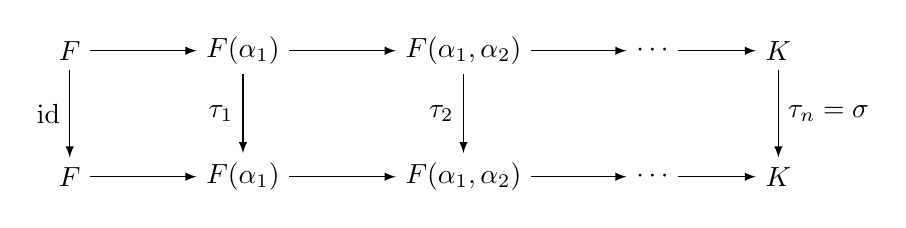
\begin{tikzpicture}[>=latex]
  \node (F)  at (0,1.6)   {$F$};
  \node (F1) at (2.2,1.6) {$F(\alpha_1)$};
  \node (F2) at (5.0,1.6) {$F(\alpha_1,\alpha_2)$};
  \node (dots) at (7.4,1.6) {$\cdots$};
  \node (K)  at (9.0,1.6) {$K$};
  \node (G)  at (0,0)   {$F$};
  \node (G1) at (2.2,0) {$F(\alpha_1)$};
  \node (G2) at (5.0,0) {$F(\alpha_1,\alpha_2)$};
  \node (gdots) at (7.4,0) {$\cdots$};
  \node (K2) at (9.0,0) {$K$};
  \draw[->] (F) -- (F1);
  \draw[->] (F1) -- (F2);
  \draw[->] (F2) -- (dots);
  \draw[->] (dots) -- (K);
  \draw[->] (G) -- (G1);
  \draw[->] (G1) -- (G2);
  \draw[->] (G2) -- (gdots);
  \draw[->] (gdots) -- (K2);
  \draw[->] (F) -- (G) node[midway,left] {$\mathrm{id}$};
  \draw[->] (F1) -- (G1) node[midway,left] {$\tau_1$};
  \draw[->] (F2) -- (G2) node[midway,left] {$\tau_2$};
  \draw[->] (K) -- (K2) node[midway,right] {$\tau_n=\sigma$};
\end{tikzpicture}
\end{document}
